\chapter{Методы прогнозирования}

Под прогнозированием, в широком смысле, понимают предсказание
будущего с помощью научных методов~\cite{myref9}.
Необходимо различать два взаимосвязанных понятия -- метод прогнозирования и модель прогнозирования.

\textit{Метод} прогнозирования представляет собой последовательность действий, которые нужно совершить для получения модели прогнозирования временного ряда~\cite{myref12}.

\textit{Модель} прогнозирования есть представление зависимости будущего значения от прошлого~\cite{myref9, myref13},
при этом способ задания этой зависимости может быть различным.

В \textit{статистических} моделях функциональная зависимость между
будущими и фактическими значениями временного ряда, а также
внешними факторами \textit{задана аналитически}~\cite{myref9}.

К статистическим относятся следующие группы моделей:

\begin{itemize}
\item регрессионные;
\item авторегрессионные;
\item экспоненциального сглаживания~\cite{myref9}.
\end{itemize}

В \textit{структурных} моделях зависимость будущего значения от прошлого задается в виде некоторой \textit{структуры} и правил \textit{перехода} по ней~\cite{myref9, myref13}.

К структурным относятся следующие группы моделей:

\begin{itemize}
\item нейросетевые;
\item на базе цепей Маркова;
\item на базе классификационно -- регрессионных деревьев~\cite{myref9}.
\end{itemize}

Необходимо отметить, что названия моделей и соответствующих методов как правило совпадают~\cite{myref9}.

На основе полученных и хранимых данных прогнозируется дальнейшее поведение временных рядов.

В нашей работе будут рассмотрены следующие методы:

\begin{itemize}
\item (модель экспоненциального сглаживания);
\item модель на цепях Маркова;
\item( регрессионная модель):
    \begin{itemize}
        \item (простая линейная регрессия);
        \item (множественная регрессия);
        \item (нелинейная регрессия);
    \end{itemize}
\item авторегрессионные модели:
\begin{itemize}
    \item (ARIMAX);
    \item (GARCH);
    \item (ARDLM);
    \item модель по выборке максимального подобия;
\end{itemize}
\item (модель на классификационно -- регрессионных деревьях(CART))~\cite{myref9}.
\end{itemize}


\section{Модель на цепях Маркова}

\textit{Цепь Маркова} --- это математическая модель, которая используется для моделирования случайных процессов,
происходящих в течение определенного периода времени~\cite{myref8, myref9, myref13, myref16}.
Она состоит из набора состояний и переходов между ними~\cite{myref16, myref9}.
Возможность перехода из одного состояния в другое зависит исключительно от текущего состояния, а не от каких-либо прошлых событий.
Данное условие также называют марковским свойством процесса~\cite{myref8, myref9,myref13, myref16}.

Пример цепи Маркова для процесса, имеющего три состояния, представлен на рисунке~\ref{chain}, где $S1$, $S2$, $S3$ — состояния процесса $Z(t)$,
а вероятность перехода из состояния:
\begin{itemize}
    \item S1 в S2 равна 0.5,
    \item S2 в S1 равна 0.0,
    \item S1 в S3 равна 0.25,
    \item S3 в S2 равна 0.33 и так далее.
\end{itemize}

\begin{figure}[h]
    \centering
    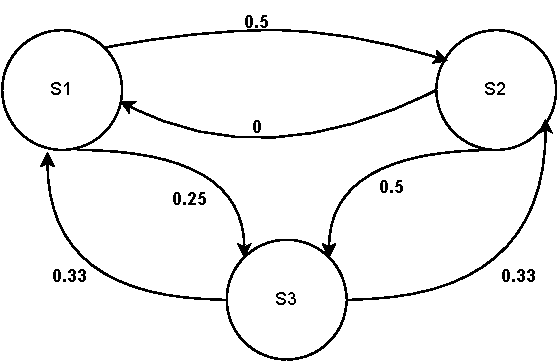
\includegraphics[scale=1.1]{img/chain}
    \caption{Цепь Маркова}
    \label{chain}
\end{figure}

Для расчета динамики цепи достаточно рассмотреть два аспекта:
\begin{itemize}
    \item \textit{вектор исходного распределения вероятностей} $A$ ---
    вектор, каждое $i$-ое значение в котором, соответствует вероятности того, что система находится в $i$-ом состоянии~\cite{myref1}.
    Например, для модели из трех состояний:
    \begin{equation}
        A = (0.0, 0.5, 0.5);
        \label{eq:equation2}
    \end{equation}
    \item матрицу переходных вероятностей $P$, представляющую собой матрицу, каждое значение $(i, j)$ которой
    соответствует вероятности того, что элемент перейдет из состояния $s_i$ в состояние $s_j$ на следующем шаге процесса~\cite{myref1}.
    Например, для модели на рисунке выше:
    \begin{equation}
        P = \begin{pmatrix}0.25, 0.50, 0.25\\
        0.00, 0.50, 0.50\\
        0.33, 0.33, 0.33
        \end{pmatrix}.
        \label{eq:equation3}
    \end{equation}
\end{itemize}

Чтобы определить вектор распределения вероятностей на следующем шаге необходимо вычислить произведение вектора $A$ и матрицы $P$~\cite{myref13}.
Для рассматриваемого примера:

\begin{equation}
(0.00, 0.50, 0.50) = \begin{pmatrix}0.25, 0.50, 0.25\\
0.00, 0.50, 0.50\\
0.33, 0.33, 0.33
\end{pmatrix}=(0.165, 0.415, 0.420).
\label{eq:equation4}
\end{equation}

Следовательно, вероятность того, что цепь находится в состоянии $s_i$ после $n$ шагов, является $i$-ой записью в векторе~\cite{myref1}:
\begin{equation}
    A_n = A_{n-1}P.
    \label{eq:equation5}
\end{equation}

Основные этапы алгоритма построения модели временного ряда на цепях Маркова:
\begin{enumerate}
    \item выделить состояния временного ряда;
    \item проверить, можно ли считать рассматриваемый процесс Марковским;
    \item вычислить матрицу переходных вероятностей;
    \item определить вероятностный вектор, представляющий некоторое начальное распределение;
    \item вычислить произведение матрицы и вектора n раз для получения вектора распределения вероятностей.
\end{enumerate}

Рассмотрев метод прогнозирования на цепях Маркова, выделим следующие особенности его применения:
\begin{itemize}
    \item необходимо выделить состояния временного ряда.
    Данное действие является дополнительным и зависит от сферы применения временного ряда;
    \item прогнозируемый ряд должен являться Марковским процессом;
    \item единообразие анализа и проектирования~\cite{myref9}.
\end{itemize}

\section{Модель по выборке максимального подобия EMMSP}

Для удобства анализа данной модели временной ряд обозначим как $Z_1^N=(z_1,z_2,\ldots,z_N)$.
Набор из $M$ последовательных значений \newline $Z_t^M=(z_t,z_{t+1},\ldots,z_{t+M-1})$, лежащих внутри временного ряда $Z_1^N$,
назовем \textit{выборкой} из этого ряда длины $M\in[1,(N-1)]$ с моментом начала отсчета $t\in[1,(N-M)]$.
Разность начал отсчетов выборок $Z_t^M$ и $Z_{t-k}^M$ будем называть \textit{задержкой} $k\in[1,(t-1)]$.

Выборки обладают свойством подобия, чем мы и воспользуемся для прогнозирования временного ряда~\cite{myref9}.
Идея метода заключается в построении ожидаемой выборки с помощью аппроксимации уже существующей.
С целью реализации данной технологии следует ответить на следующие вопросы.

1. Как аппроксимировать выборки?

Рассмотрим аппроксимацию выборки \newline $Z_{T-M+1}^M$ при помощи выборки $Z_{T-M+1-k}^M$~\cite{myref9}.
Обозначим момент времени $T-M+1=t$.

Вычислим аппроксимированные значения выборки $\widehat{Z}_t^M$:

\begin{equation}
    \widehat{Z}_t^M = \alpha_1Z_{T-k}^M+\alpha_0I^M,
\end{equation}
где $\alpha_1$ и $\alpha_0$ --- коэффициенты,
а $I^M$ - единичный вектор размерности $M$.

Согласно методу наименьших квадратов, коэффициенты аппроксимации определим, исходя из уравнения

\begin{equation}
    Z_x \cdot A = Z_y,
\end{equation}

где $Z_x$ и $Z_y$ определяются следующим образом:
\begin{flushright}
\begin{equation}
    Z_X =
\begin{pmatrix}
           \sum_{i=0}^{M-1} Z^2(k+1) & \sum_{i=0}^{M-1} Z(k+i) \\
           \sum_{i=0}^{M-1} Z(k+1)   & M
\end{pmatrix};

    Z_Y =
    \begin{pmatrix}
               \sum_{i=0}^{M-1} Z(k+i) \cdot Z(T-M+1+i) \\
               \sum_{i=0}^{M-1} Z(T-M+1+i)
\end{pmatrix}.{\qquad\qquad }
    \label{eq:equation}
\end{equation}
\end{flushright}

2. Какую выборку следует аппроксимировать?

Подходящую для аппроксимации выборку называют \textit{базовой историей}~\cite{myref9}.
Она располагается на оси времени сразу за \textit{выборкой максимального подобия} для новой истории $Z_{T-M+1}^M$~\cite{myref9}.
Новая история содержит значения процесса непосредственно перед моментом прогноза.
Соответственно, чтобы вычислить базовую историю, следует определить выборку максимального подобия.

3. Как определить выборку максимального подобия для выборки новой истории?

Как следует из названия, мы ищем такую выборку, значения которой являются наиболее близкими к значениям новой истории.
Отсюда, необходимо ввести меру подобия двух выборок.
Введем коэффициент $\rho$.
Он зависит от длины $M$ выборок, а также от задержки $k$, и характеризует степень линейной зависимости указанных выборок:
чем ближе к единице значение $\rho$, тем выше их линейная зависимость~\cite{myref9, myref11}.

Далее необходимо рассмотреть все возможные выборки длины $M$ и вычислить для них коэффициент подобия новой истории.
Выборка с максимальным значением $\rho$ и будет выборкой максимального подобия.
Данной выборке соответствует задержка $k$, которую далее обозначим как $kmax$.

В результате получаем функциональную зависимость значений прогнозируемой выборки $Z_t^P$ от фактически существующей $Z_{T-k}^M$~\cite{myref9}:

\begin{equation}
    \widehat{Z}_t^P = \alpha_1Z_{k_{max}+M}^P+\alpha_0I^P=EMMSP(M),
\end{equation}

На рисунке~\ref{img2} приведен пример расположения рассмотренных для прогнозирования выборок.
\begin{figure}[h]
    \centering
    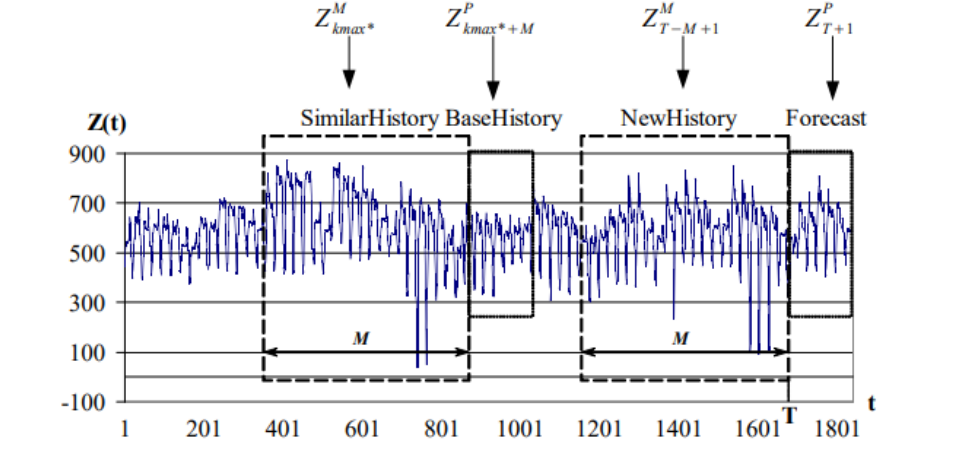
\includegraphics[scale=0.7]{img/img2}
    \caption{Положение выборок для прогнозирования временного ряда с помощью модели по выборке максимального подобия без учета внешних факторов~\cite{myref9}}
    \label{img2}
\end{figure}

Кроме того, существует возможность построить модель, учитывающую внешние факторы,
которые также представлены в виде временного ряда со значениями, соответствующими отметкам времени временного ряда $Z$.
В данной модели отличается процесс аппроксимации выборок, в остальном алгоритм прогнозирования аналогичен уже рассмотренному.

Функциональная зависимость значений прогнозируемой выборки $Z_t^P$ от фактически существующей $Z_{T-k}^M$,
с учетом внешних факторов $X$, будет выглядеть следующим образом~\cite{myref9}:

\begin{equation}
    \widehat{Z}_{T+1}^P = \alpha_2Z_{k_{max^*+M}+M}^P+\alpha_0I^P+\alpha_1X_{T+1}^P=EMMSP(M),
\end{equation}

На рисунке~\ref{img3} представлены выборки для модели с учетом внешних факторов.
\begin{figure}[h]
    \centering
    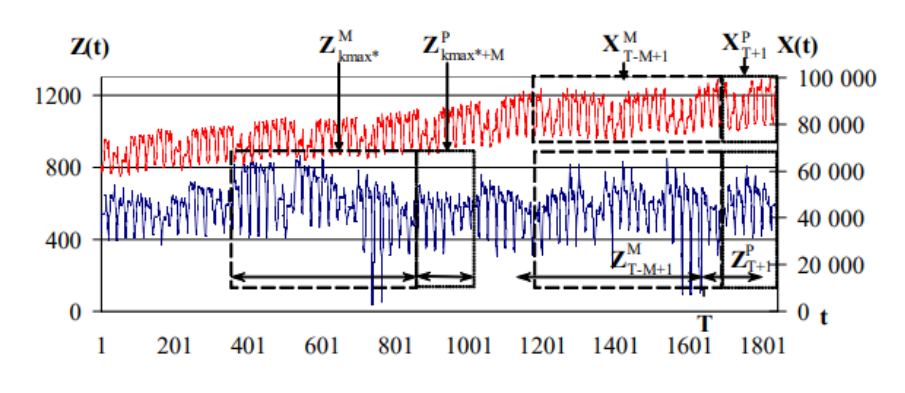
\includegraphics[scale=0.8]{img/img3}
    \caption{Положение выборок для прогнозирования временного ряда с помощью модели по выборке максимального подобия с учетом внешних факторов~\cite{myref9}}
    \label{img3}
\end{figure}


Подводя итоги, можно выделить основные этапы алгоритма построения модели по выборке максимального подобия.

Необходимо вычислить:
\begin{enumerate}
    \item выборку новой истории;
    \item выборку максимального подобия;
    \item выборку базовой истории;
    \item прогнозные значения.
\end{enumerate}

Рассмотрев метод прогнозирования по выборке максимального подобия, можно выделить следующие особенности его применения:

\begin{itemize}
    \item модель работает с неравноотстоящими временными рядами;
    \item модель применяется для стационарных и нестационарных временных рядов;
    \item количество итераций (1шт.) для вычисления прогноза не зависит от требуемого количества элементов прогнозируемой выборки;
    \item модель имеет единственный параметр $M$ --- длина выборки, от которого зависит значение прогнозируемого участка, в отличие от других авторегрессионных моделей.
\end{itemize}

\section{Выводы}

Результаты сравнения двух методов прогнозирования временных
рядов приведены в таблице~\ref{tab_prog}

\begin{table}[h!]
    \caption{Сравнения двух методов прогнозирования временных рядов на модели по выборке максимального подобия и модели на Марковских цепях}
    \label{tab_prog}
    \centering
    \begin{tabular}{||p{5cm}|p{5cm}|p{5cm}||}
        \hline
        параметр / метод и модель & модель на цепях Маркова & Модель по подборке максимального подобия\\
        \hline \hline
        {тип модели} & структурная & статическая \\
        \hline
        {необходимость преобразовывать данные временного ряда перед их прогнозированием} & есть & нет\\
        \hline
        {количество итераций или раз применения некоторой формулы для получения прогноза} & $n$ раз для прогнозирования n состояний & одна итерация. Однако перед этим проводится аппроксимация Т-М-1 выборок длины М. \\
        \hline
        {область применения} &  {применимо к временным рядам, выполняющим Марковское свойство. Неприменимо к долгохранимым временным рядам} & Неравностоящие, стационарные и нестационарные ряды \\
        \hline
        {Количество параметров, влияющих на результат, задаваемых пользователем} & 0 & 1 --- длина выборки М \\
        \hline \hline
    \end{tabular}
\end{table}
\clearpage

Анализ представленных в таблице данных позволяет сделать
следующие выводы:
\begin{itemize}
    \item область применения методов построения модели на Марковских цепях
и модели по выборке максимального подобия различны: в некоторых
ситуациях можно использовать первую модель, в то время как вторая
будет неприменима и наоборот;
    \item метод на Марковских цепях требует дополнительных проверок перед
его применением;
    \item модель на Марковских цепях требует анализа временных рядов и их
преобразования - выделения состояний;
    \item количество необходимых вычислений для прогнозирования временных
рядов варьируется. Для краткосрочных прогнозов использование
модели на Марковских цепях предпочтительнее, так как количество
итераций (перемножений матрицы и вектора) будет равно количеству
прогнозируемых состояний, в то время как в модели по выборке
максимального подобия количество итераций будет равно Т-М-1, где Т
- количество значений временного ряда, а М - длина выборки.
\end{itemize}